\documentclass[12pt]{beamer}
\usepackage{pgf}
\usepackage[danish]{babel}
\usepackage[utf8]{inputenc}
\usepackage{beamerthemesplit}
\usepackage{graphics,epsfig, subfigure}
\usepackage{url}
\usepackage{srcltx}
\usepackage{hyperref}
\usepackage{fancybox}
\usepackage{listings}
\lstset{
  language=C,                % choose the language of the code
   basicstyle=\footnotesize,        % the size of the fonts that are used for the code
    keywordstyle=\color{blue},       % keyword style
     commentstyle=\color[rgb]{0.13,0.54,0.13},
  numbers=left,                   % where to put the line-numbers
  stepnumber= 0.3,                   % the step between two line-numbers.        
  numbersep=1pt,                  % how far the line-numbers are from the code
  backgroundcolor=\color{white},  % choose the background color. You must add \usepackage{color}
  showspaces=false,               % show spaces adding particular underscores
  showstringspaces=false,         % underline spaces within strings
  showtabs=false,                 % show tabs within strings adding particular underscores
  tabsize=2,                      % sets default tabsize to 2 spaces
  captionpos=b,                   % sets the caption-position to bottom
  breaklines=true,                % sets automatic line breaking
  breakatwhitespace=true,         % sets if automatic breaks should only happen at whitespace
 % title=\lstname,                 % show the filename of files included with \lstinputlisting;
}
\definecolor{kugreen}{RGB}{50,93,61}
\definecolor{kugreenlys}{RGB}{132,158,139}
\definecolor{kugreenlyslys}{RGB}{173,190,177}
\definecolor{kugreenlyslyslys}{RGB}{214,223,216}
\setbeamercovered{transparent}
\mode<presentation>
\usetheme[numbers,totalnumber,compress,sidebarshades]{PaloAlto}
\setbeamertemplate{footline}[frame number]

  \usecolortheme[named=kugreen]{structure}
  \useinnertheme{circles}
  \usefonttheme[onlymath]{serif}
  \setbeamercovered{transparent}
  \setbeamertemplate{blocks}[rounded][shadow=true]

\logo{
\includegraphics[width=0.8cm]{fga_logo.png}}
%\useoutertheme{infolines} 
\title{Métodos de Desenvolvimento de Software}
\author{Dra. Carla Rocha, Msc. Hilmer Neri}
\institute{Engenharia de Software \\ Universidade de Brasília}
\date{}

\begin{document}
\frame{\titlepage \vspace{-0.5cm}
}
\frame
{
\frametitle{Agenda}
\tableofcontents%[pausesection]
}

\section{Engenharia de Software}

\begin{frame}
\begin{block}{Processo de Software}
 \textit{”Software processes are software, too,” wrote Lee Osterweil.1}
\end{block}
\end{frame}


\begin{frame}
\frametitle{Uma abordagem de engenharia:\\
Construção de uma casa}

\begin{figure}
  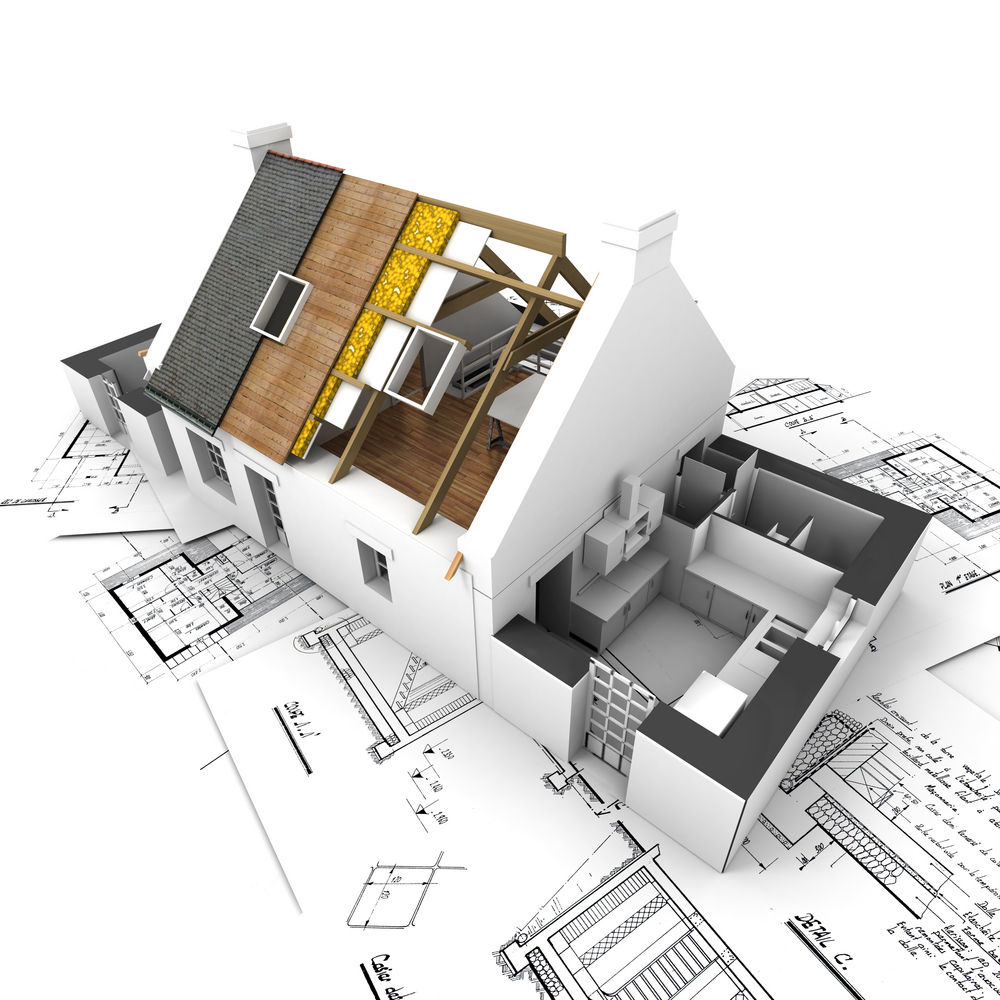
\includegraphics[height = \textheight]{figs/construcao-de-moradia.jpg}
 \end{figure}

\end{frame}

\begin{frame}
\frametitle{Uma abordagem de engenharia:\\
Construção de uma casa}
\begin{itemize}
 \item Equipes grandes e habilidades específicas
%\pause
 \item Os clientes explicam o que querem (aparência, características)
%\pause
 \item A construtora apresenta um projeto arquitetônico e um plano de construção
 %\pause
\item São feitas mudanças e o projeto é finalmente aprovado
\end{itemize}
\end{frame}


\begin{frame}
\frametitle{Uma abordagem de engenharia:\\
Construção de uma casa}
\begin{itemize}
 \item Inspeções da obra e novas mudanças
podem ocorrer
%\pause
\item Durante a construção, vários componentes
serão testados: circuitos elétricos,
encanamentos, nivelamento do
madeiramento
%\pause
\item Finalmente, os clientes se mudam para a
casa
\end{itemize}
\end{frame}

\section{Processos de Software}
\begin{frame}
\frametitle{Uma abordagem de engenharia:\\
Processo de Construção}
\begin{itemize}
 \item Muitas pessoas na obra, é necessário documentação.
%\pause
\item Integrar os produtos (elétrico x hidráulico x estrutural)
%\pause

\item Não é esperado que os clientes descrevam a
casa totalmente no início do processo. Mudanças ocorrem durante a construção

%\pause
\item A construtora deve fornecer plantas, diagramas elétricos, planta hidráulica, manuais
\end{itemize}
\end{frame}

\begin{frame}
\frametitle{Uma abordagem de engenharia:\\
Processo de Construção}
\begin{itemize}
\item Identificar e analisar os requisitos
%\pause
\item Produzir e documentar o projeto da casa
%\pause
\item Produzir as especificações detalhadas da casa
%\pause
\item Identificar e projetar os componentes
%\pause
\item Construir cada componente da casa
%\pause
\item Testar cada componente da casa
%\pause
\item Integrar os componentes e realizar modificações finais
%\pause
\item Manutenção contínua pelos moradores da casa
\end{itemize}
\end{frame}



\begin{frame}
\frametitle{Engenharia de Software}
\begin{itemize}
\item Problemas x solução
%\pause
\item Algo novo é difícil de resolver
%\pause
\item  Iniciar com a \textbf{análise} do problema
\begin{itemize}
 \item Dividir em partes para facilitar entendimento
\end{itemize}
\end{itemize}
\end{frame}

\begin{frame}
 \begin{figure}
  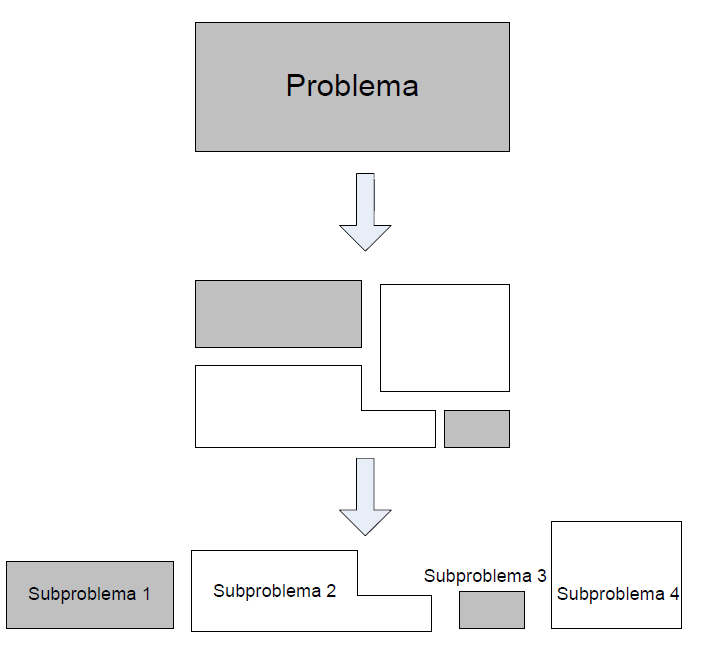
\includegraphics[height = \textheight]{figs/fig1.png}
 \end{figure}

\end{frame}


\begin{frame}
\frametitle{Engenharia de Software}
\begin{itemize}
\item Para solucionar o problema: métodos,
ferramentas, procedimentos e paradigmas
\begin{itemize}
 \item Método : técnica formal para produzir um
resultado
%\pause
\item Ferramenta: instrumento para realizar uma tarefa
da melhor maneira
%\pause
\item Procedimento: combinação de ferramentas e técnicas
%\pause
\item Paradigma: abordagem para a construção do software
\end{itemize}
\end{itemize}
\end{frame}

\begin{frame}
\frametitle{Engenharia de Software x \\ Engenharia da Computação}
\begin{itemize}
\item Podemos nos concentrar nos computadores
ou linguagens de programação por eles mesmos; ou
%\pause
\item Vê-los como ferramentas a serem utilizadas
no projeto e na implementação da solução de um problema.
\end{itemize}
\end{frame}

\begin{frame}
\frametitle{Engenharia de Software x \\ Engenharia da Computação}
\begin{figure}
 \centering
 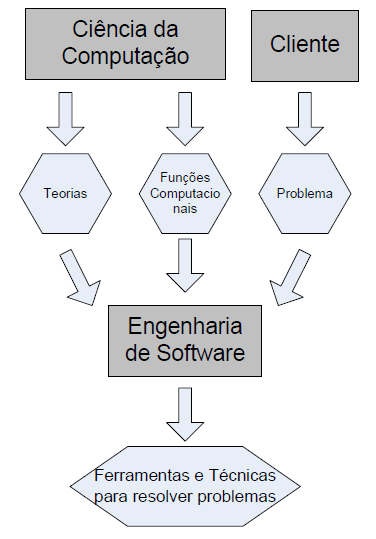
\includegraphics[height = \textheight]{figs/fig2.png}
\end{figure}
\end{frame}

\begin{frame}
 \frametitle{Engenharia de Software}
 \begin{itemize}
  \item Usa abordagens sistemáticas, econômicas e quantificáveis para o desenvolvimento, operação e manutenção de software.
 \end{itemize}
\begin{block}{Objetivo}
 O objetivo é fornecer uma estrutura para a construção de \textbf{software com alta qualidade}.
\end{block}
\begin{figure}
 \centering
 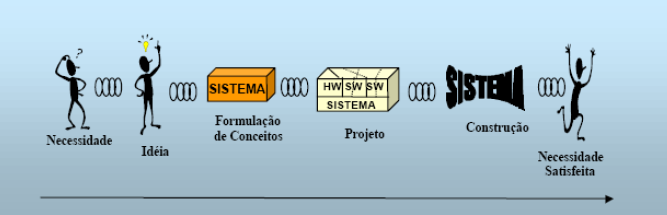
\includegraphics[width = 0.7\textwidth]{figs/fig3.png}
\end{figure}
\end{frame}


\begin{frame}
 \frametitle{Qualidade de Software}
 \begin{itemize}
  \item Engenheiros de software buscam métodos para assegurar a qualidade no software que
produzem será util
%\pause
\begin{itemize}
 \item Qualidade do produto
 \item Qualidade do processo
 \item  Qualidade do produto no ambiente de negócios que será utilizado.
\end{itemize}
 \end{itemize}
\end{frame}

\section{Método x Metologia}
\begin{frame}
 \frametitle{Método}
 \begin{center}
  \begin{block}{}
  É o caminho pelo qual fazemos algo, de maneira a atingir um objetivo; exige a
organização do conhecimento e experiências prévias.(LEOPARDI, 1999) 
  \end{block}
 \end{center}
\end{frame}

\begin{frame}
 \frametitle{Metodologia}
 \begin{center}
  \begin{block}{}
   Disciplina que se ocupa de estudar e ordenar (no possível) os muitos métodos que
concebemos, suas origens históricas, seus embasamentos paradigmáticos
acompanhados de suas relações teóricas, suas características estruturais e as
especificidades de seus alvos. (TURATO,2003:153)
  \end{block}
 \end{center}
\end{frame}

\begin{frame}
 \frametitle{Etmologia das palavras}
 \begin{itemize}
  \item Methodos = “Caminho para se chegar a um fim”
  %\pause
  \item logia = “Estudo de”
 \end{itemize}
\end{frame}

\begin{frame}
 \frametitle{Na Engenharia de Software}
 \begin{itemize}
  \item \textbf{Métodos}: técnica formal para produzir um
resultado.
%\pause
\item \textbf{Metodologia}: Uma abordagem filosófica do
problema. Ex: metodologia estruturada, metodologias ágeis, metodologia orientada a
objetos, etc.
 \end{itemize}
\end{frame}

\begin{frame}
 \frametitle{Processo}
 \begin{itemize}
  \item Uma série de etapas que envolve atividades que transforma entradas (insumos) em
saídas (produtos).
%\pause
\item Envolve um conjunto de técnicas (métodos) e ferramentas, restrições e recursos.
 \end{itemize}
\begin{figure}
 \centering
 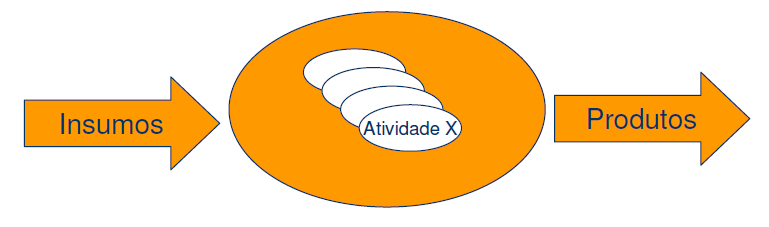
\includegraphics[height = 0.4\textheight]{figs/fig4.png}
\end{figure}
 \end{frame}

 \begin{frame}
  \frametitle{Procedimento x Processo}
  \begin{itemize}
   \item \textbf{Procedimento}: como uma receita, uma
maneira estruturada de combinar ferramentas e técnicas para gerar um
resultado 
%\pause
\item \textbf{Processo}: Conjunto de procedimentos organizados de forma a permitir construir
produtos que satisfaçam objetivos e padrões
  \end{itemize}
 \end{frame}

  \begin{frame}
  \frametitle{Procedimento x Processo}
  \begin{itemize}
   \item \textbf{Exemplo}: O processo exige que os produtos
de projeto sejam revisados antes de
codificados.
%\pause
\begin{itemize}
 \item A avaliação pode ser feita com revisões formais
ou inspeções formais.
\item Cada tipo de revisão possui um procedimento,
mas ambas com o mesmo objetivo estabelecido pelo processo.
\end{itemize}
  \end{itemize}
 \end{frame}
  
 \begin{frame}
 \frametitle{Processo de Software}
 \begin{center}
  \begin{block}{}
   Uma \textbf{estrutura comum} que define um conjunto de atividades, que são aplicáveis a
todos os projetos de software, independentemente de seu tamanho ou complexidade.
  \end{block}
 \end{center}
\begin{figure}
 \centering
 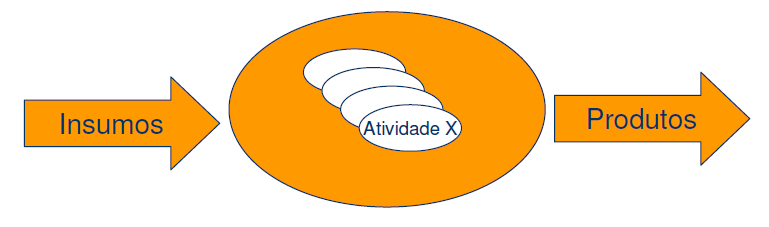
\includegraphics[height = 0.4\textheight]{figs/fig4.png}
\end{figure}
 \end{frame}
 
 \begin{frame}
  \frametitle{Por que utilizar Processos de Software?}
  \begin{itemize}
   \item Orienta as ações,permitindo examinar, entender, controlar e aprimorar as atividades
que o compõe.
%\pause
\item Capturar experiências e passá-las adiante. 
%\pause
\item  Padroniza as atividades e produtos, garante consistência e estrutura a um conjunto de
atividades.
  \end{itemize}
 \end{frame}

 \section{Disciplina}
\begin{frame}
 \frametitle{Objetivos da Disciplina}
 \begin{itemize}
  \item Estudar modelos de processos
  %\pause
  \item Estudar diferentes métodos, ferramentas e procedimentos
  %\pause
  \item Estudar processos de software já consolidados
  %\pause
  \item Exercitar em estudos de caso
 \end{itemize}
\end{frame}

\begin{frame}
 \frametitle{Objetivos da Disciplina}
 \begin{figure}
  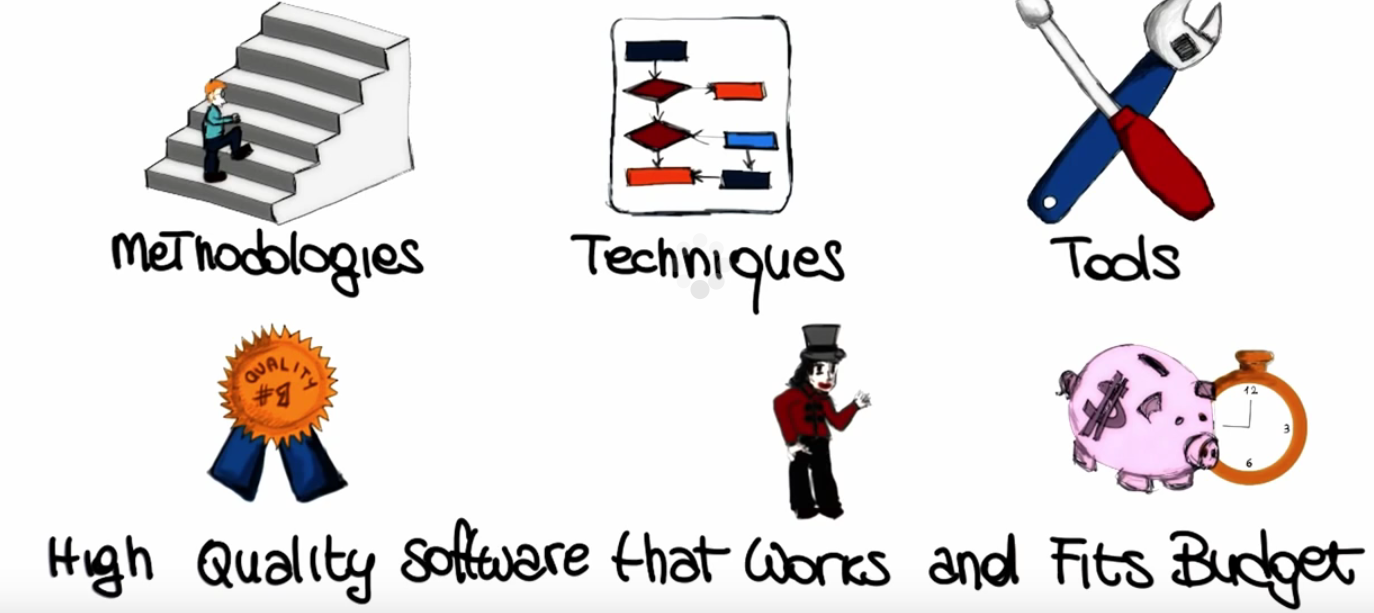
\includegraphics[width = \textwidth]{figs/fig5.png}
 \end{figure}

\end{frame}



\begin{frame}
\frametitle{Bibliografia da Aula}
\begin{itemize}
 \item Software Development Process - curso online  Udacity 

\end{itemize}
\end{frame}




\end{document}
